% hm-01-strawson.tex

\documentclass[xcolor=dvipsnames]{beamer}

\usepackage{graphicx}
% \usepackage{wrapfig}
% \usepackage{colortbl}
% \usepackage{alltt}
% \definecolor{myblue}{rgb}{0.8,0.85,1}

\mode<presentation>
{
  \usetheme{Warsaw}
  \setbeamercovered{transparent}
}
% \usecolortheme[named=OliveGreen]{structure}
\setbeamertemplate{navigation symbols}{} 
\setbeamertemplate{blocks}[rounded][shadow=true] 

\newif\ifBCITCourse
\BCITCoursetrue
\BCITCoursefalse
\newif\ifWhichCourse
\WhichCoursetrue
% \WhichCoursefalse
\ifBCITCourse
\ifWhichCourse
\newcommand{\CourseName}{Statistics for Food Technology}
\newcommand{\CourseNumber}{MATH 1441}
\newcommand{\CourseInst}{BCIT}
\else
\newcommand{\CourseName}{Calculus for Geomatics}
\newcommand{\CourseNumber}{MATH 1511}
\newcommand{\CourseInst}{BCIT}
\fi
\else
\newcommand{\CourseName}{Philosophy and Literature}
\newcommand{\CourseNumber}{PHIL 375}
\newcommand{\CourseInst}{UBC}
\fi

\title{Galen Strawson}
\subtitle{{\CourseNumber}, {\CourseInst}}

\author{\CourseName}

\date{September 14, 2017}

% \begin{frame}
%   \frametitle{iClicker Question One}
% Choose from the following options. This item will be graded.
% \begin{block}{iClicker Question}
  
% \end{block}
% \begin{description}
% \item[A\hspace{.2in}$\blacktriangleright$] 
% \item[B\hspace{.2in}$\blacktriangleright$] 
% \item[C\hspace{.2in}$\blacktriangleright$] 
% \item[D\hspace{.2in}$\blacktriangleright$] 
% \item[E\hspace{.2in}$\blacktriangleright$] 
% \item[F\hspace{.2in}$\blacktriangleright$] 
% \end{description}
% \end{frame}

% \begin{figure}[h]
% \includegraphics[scale=.3]{./extrema1.png}
% \end{figure}

\begin{document}

\begin{frame}
  \titlepage
\end{frame}

% \begin{frame}
%   \frametitle{Structuralism Table}
% \begin{figure}[h]
% 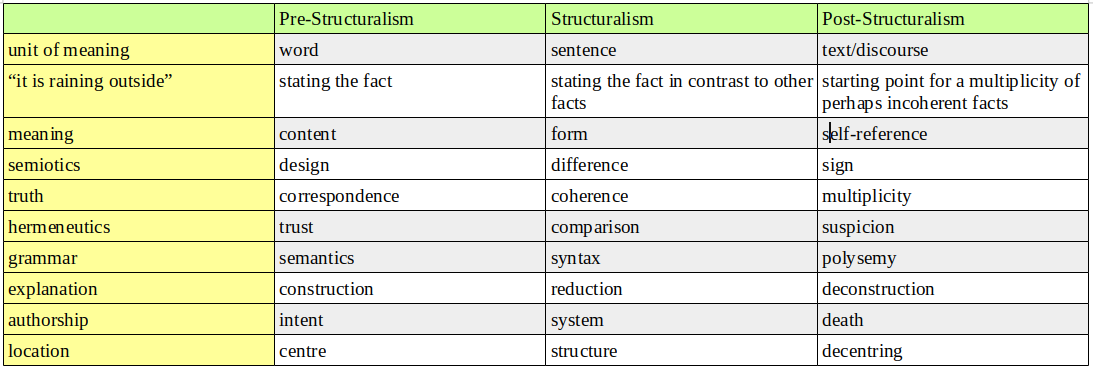
\includegraphics[scale=.3]{./structable.png}
% \end{figure}
% \end{frame}

\begin{frame}
  \frametitle{iClicker Question}
Choose from the following options. This item will not be graded.
\begin{block}{iClicker Question}
Which of the following features is not one that Galen Strawson
investigates as a possible condition for diachronicity?
\end{block}
\begin{description}
\item[A\hspace{.2in}$\blacktriangleright$] form-finding
\item[B\hspace{.2in}$\blacktriangleright$] story-telling tendency
\item[C\hspace{.2in}$\blacktriangleright$] journalling
\item[D\hspace{.2in}$\blacktriangleright$] revision
\end{description}
\end{frame}

\begin{frame}
  \frametitle{iClicker Question}
Choose from the following options. This item will not be graded.
\begin{block}{iClicker Question}
Who is Strawson's example of someone who thinks that the psychological
narrativity thesis is true (ordinary human beings experience their
lives in some sort of narrative way), but the ethical narrativity
thesis is NOT true (the narrative outlook is not essential to a
well-lived life)?
\end{block}
\begin{description}
\item[A\hspace{.2in}$\blacktriangleright$] Henry James
\item[B\hspace{.2in}$\blacktriangleright$] Jean-Paul Sartre
\item[C\hspace{.2in}$\blacktriangleright$] Marya Schechtman
\item[D\hspace{.2in}$\blacktriangleright$] Charles Taylor
\end{description}
\end{frame}

\begin{frame}
  \frametitle{iClicker Question}
Choose from the following options. This item will not be graded.
\begin{block}{iClicker Question}
What does NOF stand for?
\end{block}
\begin{description}
\item[A\hspace{.2in}$\blacktriangleright$] No Ownership of the Future
\item[B\hspace{.2in}$\blacktriangleright$] No Ordinary Family
\item[C\hspace{.2in}$\blacktriangleright$] Net Overall Futility
\item[D\hspace{.2in}$\blacktriangleright$] Never OK to Fear
\end{description}
\end{frame}

\begin{frame}
  \frametitle{iClicker Question}
Choose from the following options. This item will not be graded.
\begin{block}{iClicker Question}
Who argued that death is not an evil because it can only do harm to
someone who no longer exists?
\end{block}
\begin{description}
\item[A\hspace{.2in}$\blacktriangleright$] Gareth Evans
\item[B\hspace{.2in}$\blacktriangleright$] Marcus Aurelius
\item[C\hspace{.2in}$\blacktriangleright$] Epicurus
\item[D\hspace{.2in}$\blacktriangleright$] Jeff McMahan
\end{description}
\end{frame}

\begin{frame}
  \frametitle{Two Claims}
  \begin{description}
  \item[psychological thesis] this is a descriptive, empirical claim
    about the nature of ordinary human experience, where a lack of
    narrativity is pathological with respect to how ordinary that
    experience is
  \item[ethical thesis] this is a normative, ethical claim that a
    narrative outlook is essential to a well-lived life, to true or
    full personhood
  \end{description}
\end{frame}

\begin{frame}
  \frametitle{Combinations of the Two Claims}
  \begin{tabular}{|l|l|l|}\hline
    \hspace{.5in}               & \hspace{.5in}        & \hspace{.5in}  \\
                                & psychological thesis & ethical thesis \\
    \hspace{.5in}               & \hspace{.5in}        & \hspace{.5in}  \\ \hline
    \hspace{.5in}               & \hspace{.5in}        & \hspace{.5in} \\
    Sartre/Stoics               & yes                  & no             \\
    \hspace{.5in}               & \hspace{.5in}        & \hspace{.5in}  \\ \hline
    \hspace{.5in}               & \hspace{.5in}        & \hspace{.5in} \\
    Plutarch                    & no                   & yes            \\ 
    \hspace{.5in}               & \hspace{.5in}        & \hspace{.5in}  \\ \hline
    \hspace{.5in}               & \hspace{.5in}        & \hspace{.5in} \\
    Schechtman/Taylor/MacIntyre & yes                  & yes            \\ 
    \hspace{.5in}               & \hspace{.5in}        & \hspace{.5in}  \\ \hline
    \hspace{.5in}               & \hspace{.5in}        & \hspace{.5in} \\
    Strawson                    & no                   & no             \\ 
    \hspace{.5in}               & \hspace{.5in}        & \hspace{.5in}  \\ \hline
  \end{tabular}
\end{frame}

\begin{frame}
  \frametitle{Relevant Questions}
  \begin{itemize}
  \item What are persistence conditions?
  \item What is the difference between a human being and a subjectively
    experienced self?
  \item What is true about these intuitions: the chilling, empty
    deficiency of the Episodic life versus the macerated, clogged,
    excessively self-concerned, inauthentically second-order qualities
    of the Diachronic life?
  \item Does it make a difference to be explicitly or implicitly
    narrativizing?
  \end{itemize}
\end{frame}

\begin{frame}
  \frametitle{The Episodic Life}
  \begin{block}{Against Narrativity, page 433}
    I have absolutely no sense of my life as a narrative with form, or
    indeed as a narrative without form. Absolutely none. Nor do I have
    any great or special interest in my past. Nor do I have a great
    deal of concern for my future.
  \end{block}
\end{frame}

\begin{frame}
  \frametitle{More Relevant Questions}
  \begin{itemize}
  \item How is it that the from-the-inside quality of a memory can be
    detached from any sense that one is the subject of the remembered
    experience (434)?
  \item Does Strawson give a satisfying answer to what it is to have
    or be a self? Is there an abolition of selfhood lurking in the
    background? Who am I, and if so, how many? (Richard David Precht)
    See also \emph{The Ego Tunnel} by Thomas Metzinger or \emph{The
      Architecture of the Mind} by Peter Carruthers. What are the
    metaphysics of selfhood?
  \item How do you assess Strawson's argument that the ethical
    narrativity claim is associated with self-importance, religion,
    and narcissism (436f)?
  \end{itemize}
\end{frame}

\begin{frame}
  \frametitle{More Relevant Questions}
  \begin{itemize}
  \item Does the making coffee narrative scale up to larger narratives
    and propagate to higher levels; or is Strawson correct to call the
    narrativity claim about short-term plans trivial?
  \item Has Strawson addressed the problem that narrativists have with
    an invasive scientific anthopology? (See footnote 27.)
  \item How can a narrative be defined stringently? Note Strawson's
    emphasis on developmental, temporal unity and coherence.
  \item What does a personal relationship with an Episodic look like?
  \end{itemize}
\end{frame}

\begin{frame}
  \frametitle{Jacques Derrida I}
  \begin{quote}
    I understand that the question of the marriage vows was, this
    morning, considered interesting by some of you, the ``yes'' to the
    marriage, the performative ``yes'' -- ``I do'', ``I do''. This
    ``yes'' has to be repeated differently each time. If it's simply a
    record saying ``I do'' ``I do'' ``I do'' there is no fidelity. For
    this ``I do'' to be a renewed promise it has to be different each
    time, the same one and different. In order to follow the ``I do''
    today (before the priest), the ``idea'' of tomorrow should be the
    same and different {\ldots}
  \end{quote}
\end{frame}

\begin{frame}
  \frametitle{Jacques Derrida II}
  \begin{quote}
    {\ldots} They must follow one another and confirm themselves but,
    at the same time, be different. That's what the counter-signature
    is. Of course, even if I say to the same person ``I do'' tomorrow
    and after tomorrow, the fact that this ``I do'' is different, to
    some extent, means at the same time fidelity and betrayal. Indeed,
    it's a kind of perjury to say ``I do'' to someone. So that may be
    the paradox in the twin concepts of acoluthia and anacoluthon. You
    have to betray in order to be truthful. (Life After Theory, 10f)
  \end{quote}
\end{frame}

\begin{frame}
  \frametitle{Conditions of Narrativity}
  \begin{description}
  \item[diachronicity] I identify myself (the one who is the receiver
    of my subjective experiences) with the human being that I was in
    the past and that I will be in the future
  \item[form-finding] I seek for coherence, unity, and pattern in the
    temporal sequence events in my life
  \item[story-telling] I think of my life in recognizable literary
    genres
  \item[revision] I distort facts about my life so that they fit the
    kind of story that I want to tell about myself (444)
  \end{description}
\end{frame}

\begin{frame}
  \frametitle{Strawson's Shift}
  There is a marked shift on page 447 to a negative evaluation of
  narrativity. There appears to be some inconsistency between the
  pre-447 Strawson and the post-447 Strawson.
\end{frame}

\begin{frame}
  \frametitle{I Have No Future}
  Epicurus' argument that death does no harm.
  \begin{enumerate}
  \item ``Look back at time {\ldots} our birth. In this way nature
    holds before our eyes the mirror of our future after death. Is
    this so grim, so gloomy?'' (Lucretius)
  \item ``Death {\ldots} the most awful of evils, is nothing to us,
    seeing that, when we are, death is not come, and, when death is
    come, we are not.'' (Letter to Menoeceus)
  \end{enumerate}
Strawson's argument is not psychological, but philosophical. 
\end{frame}

\begin{frame}
  \frametitle{Relevant Questions}
  \begin{itemize}
  \item What are things that can be taken away from us? (Our country,
    our human rights, {\ldots})
  \item Can retributive justice be squared with Strawson's NOF? Is
    Strawson's view consistent with his father's view that reactive
    attitudes are independent of metaphysical justifications or
    entitlements and cannot be in contradiction to determinism?
  \item Does Strawson succeed in explaining regret? See Thomas Nagel's
    paper ``Death'' (1970). Keats (24) and Tolstoy (82). 
  \item Is Strawson's account of depression believable, that the
    condition's referent is the present, not the future? Is it true
    that a depressed person's desire is the cessation of the present
    rather than the future?
  \end{itemize}
\end{frame}

\end{document}
